\documentclass[journal,12pt,twocolumn]{IEEEtran}

\usepackage{setspace}
\usepackage{gensymb}
\singlespacing
\usepackage[cmex10]{amsmath}

\usepackage{amsthm}

\usepackage{mathrsfs}
\usepackage{txfonts}
\usepackage{stfloats}
\usepackage{bm}
\usepackage{cite}
\usepackage{cases}
\usepackage{subfig}

\usepackage{longtable}
\usepackage{multirow}

\usepackage{enumitem}
\usepackage{mathtools}
\usepackage{steinmetz}
\usepackage{tikz}
\usepackage{circuitikz}
\usepackage{verbatim}
\usepackage{tfrupee}
\usepackage[breaklinks=true]{hyperref}
\usepackage{graphicx}
\usepackage{tkz-euclide}

\usetikzlibrary{calc,math}
\usepackage{listings}
    \usepackage{color}                                            %%
    \usepackage{array}                                            %%
    \usepackage{longtable}                                        %%
    \usepackage{calc}                                             %%
    \usepackage{multirow}                                         %%
    \usepackage{hhline}                                           %%
    \usepackage{ifthen}                                           %%
    \usepackage{lscape}     
\usepackage{multicol}
\usepackage{chngcntr}

\DeclareMathOperator*{\Res}{Res}

\renewcommand\thesection{\arabic{section}}
\renewcommand\thesubsection{\thesection.\arabic{subsection}}
\renewcommand\thesubsubsection{\thesubsection.\arabic{subsubsection}}

\renewcommand\thesectiondis{\arabic{section}}
\renewcommand\thesubsectiondis{\thesectiondis.\arabic{subsection}}
\renewcommand\thesubsubsectiondis{\thesubsectiondis.\arabic{subsubsection}}


\hyphenation{op-tical net-works semi-conduc-tor}
\def\inputGnumericTable{}                                 %%

\lstset{
%language=C,
frame=single, 
breaklines=true,
columns=fullflexible
}
\begin{document}


\newtheorem{theorem}{Theorem}[section]
\newtheorem{problem}{Problem}
\newtheorem{proposition}{Proposition}[section]
\newtheorem{lemma}{Lemma}[section]
\newtheorem{corollary}[theorem]{Corollary}
\newtheorem{example}{Example}[section]
\newtheorem{definition}[problem]{Definition}

\newcommand{\BEQA}{\begin{eqnarray}}
\newcommand{\EEQA}{\end{eqnarray}}
\newcommand{\define}{\stackrel{\triangle}{=}}
\bibliographystyle{IEEEtran}
\raggedbottom
\setlength{\parindent}{0pt}
\providecommand{\mbf}{\mathbf}
\providecommand{\pr}[1]{\ensuremath{\Pr\left(#1\right)}}
\providecommand{\qfunc}[1]{\ensuremath{Q\left(#1\right)}}
\providecommand{\sbrak}[1]{\ensuremath{{}\left[#1\right]}}
\providecommand{\lsbrak}[1]{\ensuremath{{}\left[#1\right.}}
\providecommand{\rsbrak}[1]{\ensuremath{{}\left.#1\right]}}
\providecommand{\brak}[1]{\ensuremath{\left(#1\right)}}
\providecommand{\lbrak}[1]{\ensuremath{\left(#1\right.}}
\providecommand{\rbrak}[1]{\ensuremath{\left.#1\right)}}
\providecommand{\cbrak}[1]{\ensuremath{\left\{#1\right\}}}
\providecommand{\lcbrak}[1]{\ensuremath{\left\{#1\right.}}
\providecommand{\rcbrak}[1]{\ensuremath{\left.#1\right\}}}
\theoremstyle{remark}
\newtheorem{rem}{Remark}
\newcommand{\sgn}{\mathop{\mathrm{sgn}}}
\providecommand{\abs}[1]{\left\vert#1\right\vert}
\providecommand{\res}[1]{\Res\displaylimits_{#1}} 
\providecommand{\norm}[1]{\left\lVert#1\right\rVert}
%\providecommand{\norm}[1]{\lVert#1\rVert}
\providecommand{\mtx}[1]{\mathbf{#1}}
\providecommand{\mean}[1]{E\left[ #1 \right]}
\providecommand{\fourier}{\overset{\mathcal{F}}{ \rightleftharpoons}}
%\providecommand{\hilbert}{\overset{\mathcal{H}}{ \rightleftharpoons}}
\providecommand{\system}{\overset{\mathcal{H}}{ \longleftrightarrow}}
	%\newcommand{\solution}[2]{\textbf{Solution:}{#1}}
\newcommand{\solution}{\noindent \textbf{Solution: }}
\newcommand{\cosec}{\,\text{cosec}\,}
\providecommand{\dec}[2]{\ensuremath{\overset{#1}{\underset{#2}{\gtrless}}}}
\newcommand{\myvec}[1]{\ensuremath{\begin{pmatrix}#1\end{pmatrix}}}
\newcommand{\mydet}[1]{\ensuremath{\begin{vmatrix}#1\end{vmatrix}}}
\numberwithin{equation}{subsection}

\makeatletter
\@addtoreset{figure}{problem}
\makeatother
\let\StandardTheFigure\thefigure
\let\vec\mathbf

\renewcommand{\thefigure}{\theproblem}

\def\putbox#1#2#3{\makebox[0in][l]{\makebox[#1][l]{}\raisebox{\baselineskip}[0in][0in]{\raisebox{#2}[0in][0in]{#3}}}}
     \def\rightbox#1{\makebox[0in][r]{#1}}
     \def\centbox#1{\makebox[0in]{#1}}
     \def\topbox#1{\raisebox{-\baselineskip}[0in][0in]{#1}}
     \def\midbox#1{\raisebox{-0.5\baselineskip}[0in][0in]{#1}}
\vspace{3cm}
\title{Assignment 6}
\author{Sachinkumar Dubey - EE20MTECH11009}
\maketitle
\newpage
\bigskip
\renewcommand{\thefigure}{\theenumi}
\renewcommand{\thetable}{\theenumi}
Download all python codes from 
\begin{lstlisting}
https://github.com/sachinomdubey/Matrix-theory/Assignment6/codes
\end{lstlisting}
%
and latex-tikz codes from 
%
\begin{lstlisting}
https://github.com/sachinomdubey/Matrix-theory/Assignment6
\end{lstlisting}
\section{Problem}
(Rams 3.4.1) find the Asymptotes of the following:\\
\begin{align}
\vec{x}^T\myvec{1 & 0\\0 & -1}\vec{x}-\myvec{4 & 6}\vec{x}-6=0
\end{align}
\section{Solution}
Comparing the given equation with the form:
\begin{align}
\label{eq:conic_quad_form}
\vec{x}^T\vec{V}\vec{x}+2\vec{u}^T\vec{x}+f=0
\end{align}
We get:
\begin{align}
\vec{x}^T\myvec{1 & 0\\0 & -1}\vec{x}+2\myvec{-2 & -3}\vec{x}-6=0 \label{2.0.2}
\intertext{where,}
\vec{V}=\myvec{1 & 0 \\0 & -1}\label{eq:2.0.3}\\
\vec{u}=\myvec{-2 \\ -3}\label{eq:2.0.4}\\
f=-6\label{eq:2.0.5}
\end{align}
Here, $ \mydet{\vec{V}}=-1$. Since $ \mydet{\vec{V}}<0$ the given equation represents a hyperbola with center:
\begin{align}
\vec{c}&=-\vec{V}^{-1}\vec{u}=\myvec{2\\-3}
\end{align}

The characteristic equation of $\vec{V}$ is:
\begin{align}
\mydet{V-\lambda\vec{I}} = 0\\
\mydet{1-\lambda & 0 \\ 0 & -1-\lambda} = 0\\
\implies \lambda^2 -1 = 0
\label{eq:asymptotes_char}\\
\lambda_{1}= 1,
\lambda_{2}= -1
\end{align}
Finding the eigen vector matrix $\vec{P}$ such that $\vec{P}^T=\vec{P}^{-1}$:
\begin{align}
    \intertext{For \lambda_1=1}
    (\vec{V}-\lambda_1 \vec{I})\vec{p}
    _1=0\\
    \myvec{0 & 0 \\0 &-2 }\vec{p}_1=0 \\
    \implies \vec{p}_1=\myvec{1 \\ 0} \\
    \text{[Choosing Orthonormal eigen vectors]} \nonumber
\end{align}
For $\lambda_2=-1$
\begin{align}
    (\vec{V}-\lambda_2 \vec{I})\vec{p}_2=0\\
    \myvec{2 & 0 \\0 &0 }\vec{p}_2=0 \\
    \implies \vec{p}_2=\myvec{0 \\ 1} \\
    \text{[Choosing Orthonormal eigen vectors]} \nonumber\\
    \vec{P}=\myvec{ \vec{p}_1& \vec{p}_2}=\myvec{1&0 \\0& 1}
\end{align}

By affine transformation $\vec{x} = \vec{P}\vec{y}+\vec{c} $,  Equation \eqref{eq:conic_quad_form} can be written in the form:
\begin{align} 
\vec{y}^T\vec{D}\vec{y} =  \vec{u}^T\vec{V}^{-1}\vec{u} -f \\
\intertext{where,}
\vec{D} = \myvec{\lambda_1 & 0\\ 0 & \lambda_2},
\label{eq:quad_form_hyper}
\end{align}
Thus, we can write:
\begin{align}
    \lambda_1y_1^2 -\brak{-\lambda_2}y_1^2 = \vec{u}^T\vec{V}^{-1}\vec{u} -f \label{eq:2.0.17}
\end{align}
The equation \eqref{eq:2.0.17} represents a modified hyperbola, The equation of the asymptotes for \eqref{eq:2.0.17} is:
\begin{align} 
\myvec{\sqrt{\abs{\lambda_1}} & \pm \sqrt{\abs{\lambda_2}}}\vec{y} = 0 \label{eq2.0.21}
\end{align} 
Putting the values of $\lambda_1$ and $\lambda_2$ in equation \eqref{eq2.0.21}, we get the two asymptotes for \eqref{eq:2.0.17}:
\begin{align} 
\myvec{1 & 1}\vec{y} = 0 \\
\myvec{1 & -1}\vec{y} = 0
\end{align} 
These are the asymptotes of our modified hyperbola. The asymptotes of our original hyberbola in equation \eqref{2.0.2} can be obtained using:
\begin{align} 
\label{eq:quad_form_pair}
\myvec{\sqrt{\abs{\lambda_1}} & \pm \sqrt{\abs{\lambda_2}}}\vec{P}^T\brak{\vec{x}-\vec{c}} = 0
\label{eq:2.0.20}
\end{align} 
Putting the values of $\lambda_1$, $\lambda_2$ and $\vec{P}$  in equation \eqref{eq:2.0.20}, we get the equations of the asymptotes of the original hyperbola with center at $\Vec{c}$:
\begin{align} 
    \myvec{1 &-1}\myvec{1&0 \\0& 1}\brak{\vec{x}+\myvec{2 \\-3}}=0\\
    \implies \boxed{\myvec{1 &-1}\Vec{x}=5} \label{2.0.26}\\
    \myvec{1 & 1}\myvec{1&0 \\0& 1}\brak{\vec{x}+\myvec{2 \\-3}}=0\\
     \implies \boxed{\myvec{1 &1}\Vec{x}=-1} \label{2.0.28}
\end{align}

\begin{figure}[h!]
    \centering
    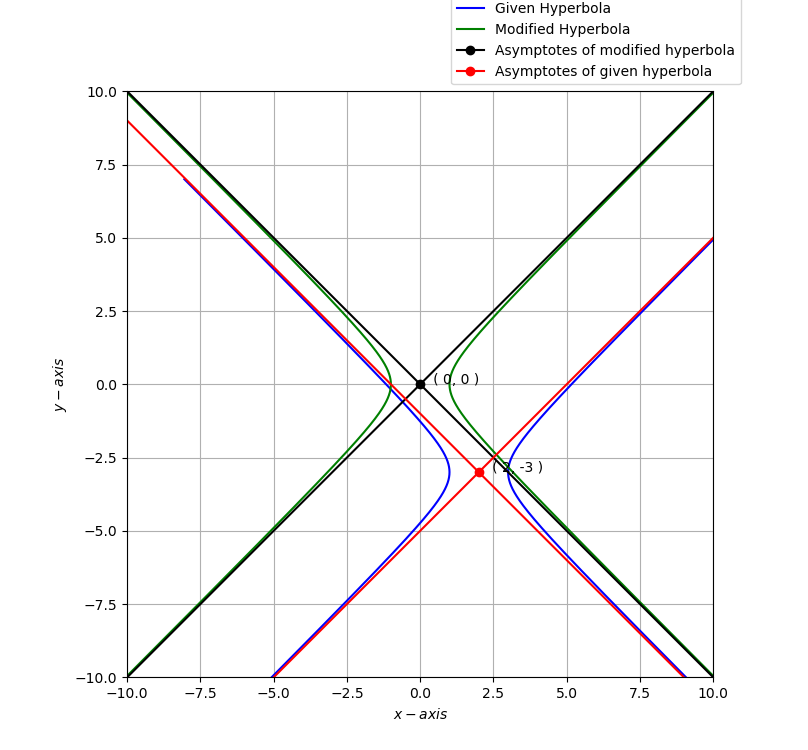
\includegraphics[width=11cm]{Figure_1.png}
    \caption{Plot of the Asymtotes.}
    \label{Plot of the Asymtotes}
\end{figure}
\end{document}